{\color{blue}
\section{Model}\label{model}

\begin{figure*}
    \centering
	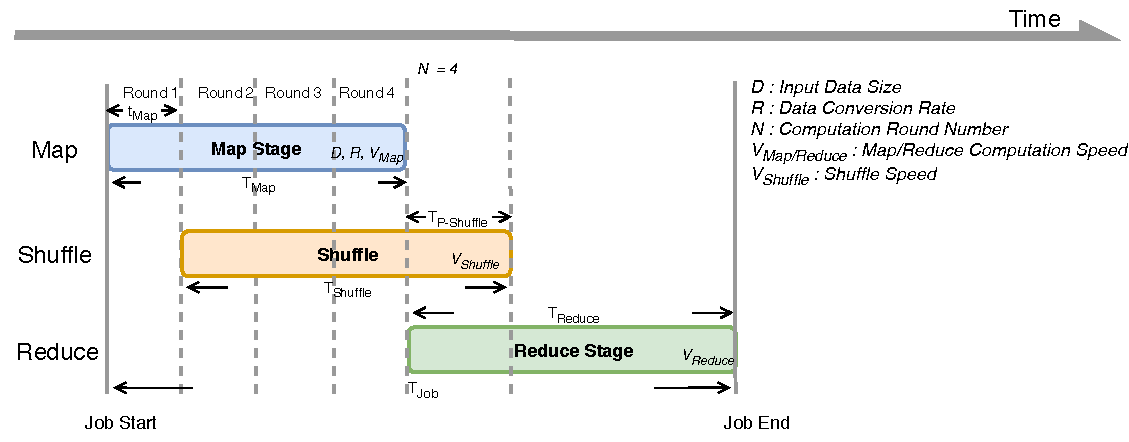
\includegraphics[width=0.85\textwidth]{fig/model_basic}
	\caption{\color{blue}??? Model}
    \label{fig:model_basic}
    \vspace{-1em}
\end{figure*}

This chapter presents a completely new model to describe the performance of distributed parallel computatino. The model analyzes the relationship between the computation stage and the shuffle stage from perspective of computation and IO resources scheduling. The model can help us evaluate the performance of the computing framework. We will first introduce model in Subsection \ref{model_overview}. In the following Subsection \ref{model_analysis}, we will use model to describe three different computation job and analyze their performance.

\subsection{Model Overview}\label{model_overview}
The current distributed parallel computation frameworks mostly use DAG(Directed acyclic graph) to describe computation logic. A shuffle stage is required between each adjacent DAG computation phase. In order to better analyze the relationship between the computation stage and the shuffle stage, we propose ??? model. ??? model describes the scheduling of computation resources and IO resources when framework is performing a computation job. ??? model can help us evaluate the performance of the framework when using different resource scheduling strategies. In this section we introduce the model by taking a simple MapReduce as an example.

Figure \ref{fig:model_basic} shows how the ??? model describes a MapReduce computing task. The model has five input parameters:
\begin{itemize}
	\item Input Data Size\((D)\): The data size of the computation stage.
	\item Data Conversion Rate\((R)\): The conversion rate of the input data to the shuffle data during a computation stage. This conversion rate depends on the algorithm used in the computation stage.
    \item Computation Round Number\((N)\): The number of rounds needed to complete the computation stage using the current computation resources. The number of rounds depends on the current computation resources and the settings of the computation job. Take Hadoop MapReduce as an example, suppose we have 50 CPUs and enough memory, the Map Stage consists of 200 map tasks. Then we need 4 rounds of computation to complete the Map phase.
    \item Computation Speed\((V_{i})\): 
    The computation speed for each computation stage. The computation speed depends on the algorithm used in the computation stage.
    \item Shuffle Speed\((V_{Shuffle})\): 
    Transmission speed during shuffle. Shuffle speed depends on Network and storage device bandwidth.
\end{itemize}

We can estimate the execution time of each stage of the job with these five parameters. Obviously, the total execution time of job in this case is the sum of the Map stage time and Reduce stage time.
\begin{equation}
\label{equation_Tjob}
\begin{aligned}
    T_{Job} &= T_{Map} + T_{Reduce}
\end{aligned}
\end{equation}
Map stage time depends on input data size and Map computation speed:
\begin{equation}
\label{equation_Tmap}
\begin{aligned}
    T_{Map} &= {{\frac{D}{V_{Map}}}}
\end{aligned}
\end{equation}
The Reduce phase time formula is as follows:
\begin{equation}
\label{equation_Treduce}
\begin{aligned}
    T_{Reduce} &= {{\frac{D \times R}{V_{Reduce}} + Overhead}}
\end{aligned}
\end{equation}
The \(Overhead\) depends on the parallel time of shuffle stage and the Reduce stage. The parallel time is denoted by \(T_{P\_Shuffle}\). The overall shuffle time is represented by \(T_{Shuffle}\). \(Overhead\) increases in proportion to \(T_{P\_Shuffle}\). This is because the computatinon of the Reduce stage relies on the data transfer results of the Shuffle stage. A portion of the computation in the Reduce stage need to wait for the transfer results. The overhead is caused by these waiting.

For shuffle-heavy computing jobs, we can optimize the job completion time by reducing \(T_{P\_Shuffle}\). Improving IO speed is a effective way to reduce shuffle time. Another optimization method is to use the idle IO resources in the Map stage for pre-fetching(see Figure \ref{fig:model_basic}). Both of the above methods can effectively reduce \(T_{P\_Shuffle}\). When using ??? model to describe a computation job, we can easily analyze the resource scheduling strategy of the computation framework. Different computing frameworks may use different resource scheduling strategies. ??? model can evaluate the scheduling strategies of these computing frameworks and help us optimize them.

\subsection{Model Analysis}\label{model_analysis}

\begin{figure}
	\centering
	\begin{minipage}[hb]{\linewidth}
		\begin{subfigure}{\linewidth}
			\begin{minipage}{\linewidth}
				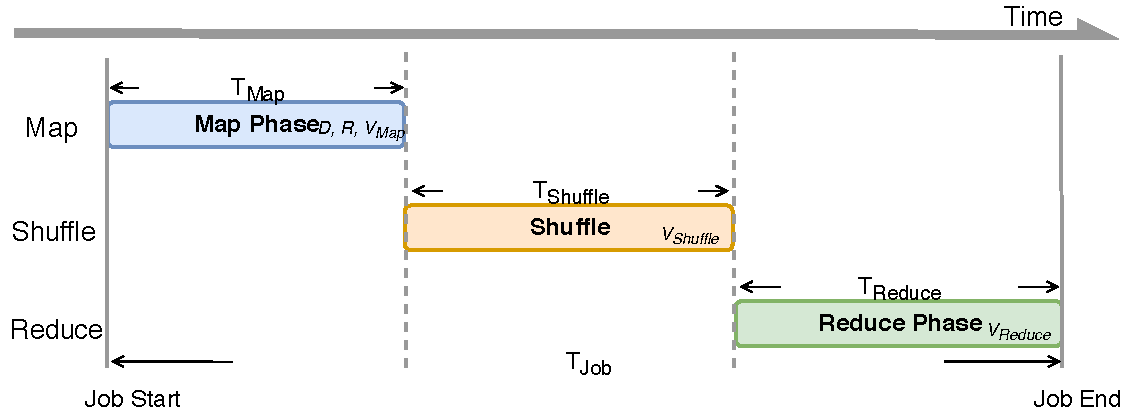
\includegraphics[width=\linewidth]{fig/model_original}
				\caption{\color{blue}Full Serial Mapreduce}
				\label{fig:model_original}
			\end{minipage}
			\begin{minipage}{\linewidth}
				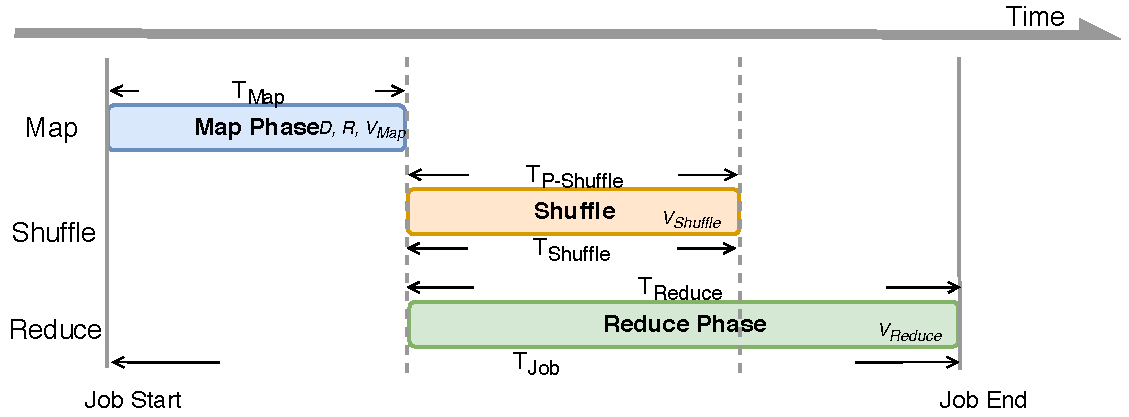
\includegraphics[width=\linewidth]{fig/model_hadoop}
				\caption{\color{blue}Hadoop Mapreduce}
				\label{fig:model_hadoop}
			\end{minipage}
		\end{subfigure}
		\caption{\color{blue}??? Model With Different Scheduling Strategies}
		\label{fig:model_strategies}
	\end{minipage}
\end{figure}

The model can describe a variety of resource scheduling strategies. First, we analyze a naive scheduling strategy. As shown in Figure \ref{fig:model_original}, the model describes a Mapreduce job that is fully serially executed. The parallel time of shuffle stage and the Reduce stage is \(0\), in which case \(T_{P\_Shuffle}\) is \(0\). Therefore, the overhead of the Reduce stage is 0. But since shuffle and computation are serial execution, the total execution time of job becomes longer:
\begin{equation}
\label{equation_Tjob}
\begin{aligned}
    T_{Job} &= T_{Map} + T_{Shuffle} + T_{Reduce}
\end{aligned}
\end{equation}
Obviously, this is an inefficient scheduling strategy. No computing framework uses this scheduling method. Due to serialization, the IO resource is idle during the Reduce stage and Map stage. The scheduling strategy is naive and has a lot of room for optimization.

Figure \ref{fig:model_hadoop} shows the scheduling strategy of Hadoop Mapreduce. In Hadoop Mapreduce, Shuffle stage and Reduce stage start at the same time. In this case, \(T_{P\_Shuffle}\) is equal to \(T_{Shuffle}\). Due to the increase in \(T_{P\_Shuffle}\), the time of Reduce phase will increase(see equation \ref{equation_Treduce}). Because the Shuffle stage and the computation stage are executed in parallel, the total execution time of job is the sum of \(T_{Map}\) and \(T_{Reduce}\)(see equation \ref{equation_Tjob}). The execution time of Shuffle stage is hidden in the Reduce stage. This scheduling strategy is much more efficient than the one in Figure 1. However, after analyzing this model, we found that the IO resource in the Map stage is idle. This scheduling strategy can be optimized.

\begin{figure}
	\centering
	\begin{minipage}[hb]{\linewidth}
		\begin{subfigure}{\linewidth}
			\begin{minipage}{\linewidth}
				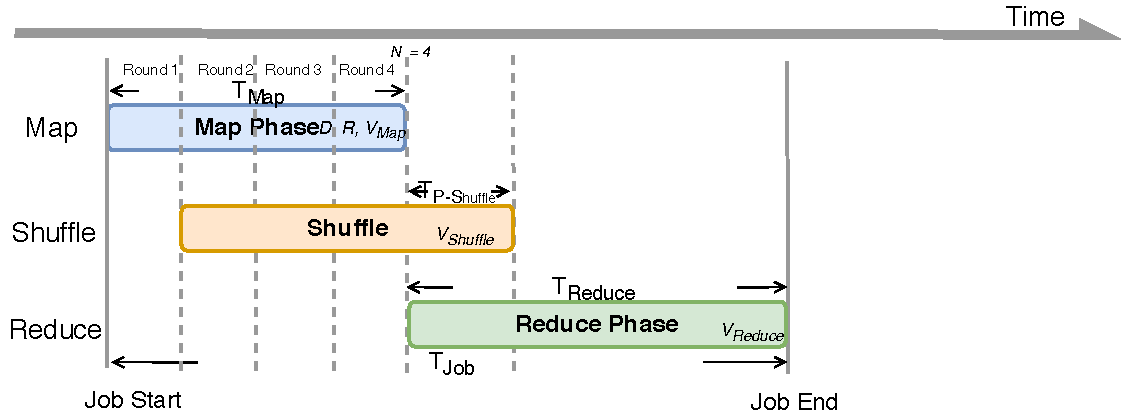
\includegraphics[width=\linewidth]{fig/model_scache1}
				\caption{\color{blue}If \(V_{Map} \times R \ge V_{Shuffle}\)}
				\label{fig:model_scache1}
			\end{minipage}
			\begin{minipage}{\linewidth}
				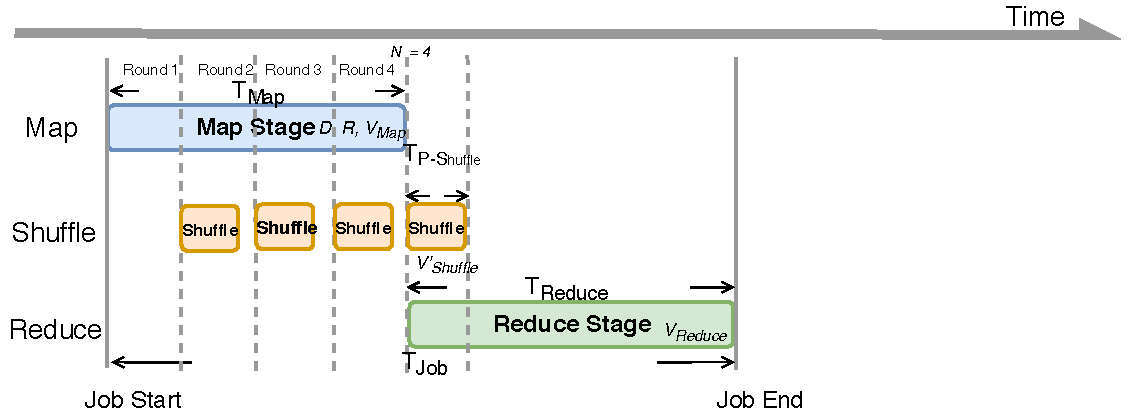
\includegraphics[width=\linewidth]{fig/model_scache2}
				\caption{\color{blue}If \(V_{Map} \times R < V_{Shuffle}\)}
				\label{fig:model_scache2}
			\end{minipage}
		\end{subfigure}
		\caption{\color{blue}??? Model With SCache}
		\label{fig:model_scache}
	\end{minipage}
\end{figure}

Figure \ref{fig:model_scache} shows the scheduling strategy for Hadoop Mapreduce with SCache (Suppose N is 4). SCache starts pre-fetching and pre-scheduling in the Map stage. This scheduling strategy can make better use of resources and avoid IO resources being idle in the Map stage. According to the experiment, we found that using the model to describe the scheduling strategy of SCache needs to distinguish two situations:

\begin{itemize}
    \item 
    \(V_{Map} \times R \ge V_{Shuffle}\)(Figure \ref{fig:model_scache1}): 
    The meaning of \(V_{Map} \times R\) is the speed at which shuffle data is generated. The meaning of the inequality is that the speed of generating shuffle data(\(V_{Map} \times R\)) is greater than or equal to the shuffle speed(\(V_{Shuffle}\)). When the Round1 of the Map phase ends, the SCache starts shuffling data until the end of the shuffle stage. Due to shuffle speed is slower, the shuffle stage is uninterrupted.
    \item \(V_{Map} \times R < V_{Shuffle}\)(Figure \ref{fig:model_scache2}): 
    When the speed of generating shuffle data(\(V_{Map} \times R\)) is less than the shuffle speed(\(V_{Shuffle}\)), SCache needs to wait for shuffle data to be generated. As Figure \ref{fig:model_scache2} shown, the shuffle stage will be interrupted in each Round.
\end{itemize}

After analyzing the above two situations, we figure out the formula for \(T_{P\_Shuffle}\):
\begin{equation}
    \label{equation_Tpshuffle}
    \begin{aligned}
    T_{P\_Shuffle} &=
        \begin{cases} 
        T_{Shuffle} - \frac{(N - 1)\times T_{Map}}{N} & , V_{Map} \times R \ge V_{Shuffle} \\ 
        T_{Shuffle} \times \frac{1}{N} & , V_{Map} \times R < V_{Shuffle}
        \end{cases}
    \end{aligned}
\end{equation}
If the shuffle speed is slow(\(V_{Map} \times R \ge V_{Shuffle}\)), SCache transmit the shuffle data generated in the last round of Map stage during the Reduce phase. Therefore \(T_{PShuffle}\) is equal to one-\(N\) of the total time of the shuffle stage. If the shuffle speed is fast (\(V_{Map} \times R < V_{Shuffle}\)), \(T_{P_Shuffle}\) is equal to the total time of shuffle (\(T_{Shuffle}\)) minus the time that shuffle is executed in the Map stage.

Compared to the original Hadoop Mapreduce resource scheduling strategy, Hadoop Mapreduce with SCache reduces \(T_{P\_Shuffle}\) and thus reduces Reduce time(\(T_{Reduce}\)). This is how pre-fetching optimizes the total execution time of job.

% \subsection{Performance Analysis}\label{model_performance_analysis}
}